\chapter{関連技術}

\section{LoRaWAN}
LoRaWANは,LoRaというSemtech社が開発した低消費電力・長距離通信用変調技術における広域ネットワーク (WAN: Wide Area Network) の規格である.LoRaWANのネットワークは,3つのコンポーネントからなり,エンドデバイス(センサノード),ゲートウェイ(GW: Gateway),アクセス制御・ネットワーク制御を行うネットワークサーバ(NS: Network Server)で構成されています.スター型のトポロジを採用し,エンドデバイスはゲートウェイを介しネットワークサーバに接続する通信モデルである.LoRaWANのデバイスは3つのカテゴリ\ref{fig:LoRaWAN}を採用している.最も利用されているのはクラスAで,消費電力が最も抑えられることや送信後の決められた時間にのみ受信が可能という特徴をもつモデルである.LoRaWANには,データレートという係数\ref{fig:LoRaWAN_DR}が7段階あり,拡散係数・伝送量・ノイズ耐性が変化する.Soracomという国内のLoRaWANプロバイダーが,ユースケース\ref{fig:LoRaWAN_Usecase}の例を挙げている.

\subsection{拡散率(SF: Spread Factor)}
LoRa物理層は,スペクトラム拡散変調(SSM: Spread Spectrum Modulation)を使用している.SSMは,高い周波数シーケンスにおいて,より広い帯域幅にわたってベース信号を拡散し,消費電力の低減,電磁妨害に対する耐性を高める.ベース信号の拡散率は可変でトレードオフであり,特定の利用可能な帯域幅に対して,より大きい拡散率はビットレートを低減させる.また,伝送時間を増加させることによってバッテリ寿命を減少させる.

\subsection{Adaptive Data Rate (ADR)}
LoRaWANの特徴でもあるAdaptive Data Rate(ADR)は、NSからセンサノードのデータレートを制御する仕組みである.センサノードの通信状況に合わせて動的に制御する.例として,センサノードとGWが近い距離にあると判断した場合,データレートを高い値に設定する.逆に、センサノードとGWが遠い距離にあると判断した場合,データレートを低い値に設定する.データレートを上げることで、送信時間が短くなり消費電力を抑えることが可能である.送信時間を短くすることに通信チャネル専有時間が削減されるためより多くのセンサノードをカバーすることが可能である.

\begin{table}[h]
    \caption{LoRaWANのクラス}\label{fig:LoRaWAN}
    \centering
    \begin{tabular}{|c|l|}
    \hline
    \multicolumn{1}{|l|}{\textbf{カテゴリ}} & \textbf{概要}                                                                                 \\ \hline
    クラスA&\begin{tabular}[c]{@{}l@{}}・消費電力が最も少ない\\ ・上り送信時のみ下り受信可能\\ ・センサデバイスの中で最も採用されている\end{tabular} \\ \hline
    クラスB                                & \begin{tabular}[c]{@{}l@{}}・消費電力がクラスAと比較し多い\\ ・スケジュールされた時刻に下り受信可能\end{tabular}              \\ \hline
    クラスC                                & \begin{tabular}[c]{@{}l@{}}・消費電力が最も多く電源があることが望ましい\\ ・双方向通信可能\end{tabular}                   \\ \hline
    \end{tabular}
\end{table}

\begin{table}[h]
    \centering
    \caption{LoRaWANのDR}\label{fig:LoRaWAN_DR}
    \begin{tabular}{|c|c|c|c|}
    \hline
    \multicolumn{1}{|l|}{\textbf{DR値}} & \multicolumn{1}{l|}{\textbf{拡散係数}} & \multicolumn{1}{l|}{\textbf{ビットレート (bps)}} & \multicolumn{1}{l|}{\textbf{受信感度 (dBm)}} \\ \hline
    DR0                                & SF12                               & 250bps                                     & -137                                     \\ \hline
    DR1                                & SF11                               & 440bps                                     & -134.5                                   \\ \hline
    DR2                                & SF10                               & 980bps                                     & -132                                     \\ \hline
    DR3                                & SF9                                & 1760bps                                    & -129                                     \\ \hline
    DR4                                & SF8                                & 3125bps                                    & -126                                     \\ \hline
    DR5                                & SF7                                & 5470bps                                    & -123                                     \\ \hline
    DR6                                & SF6                                & 11000bps                                   & -118                                     \\ \hline
    \end{tabular}
\end{table}

\begin{table}[h]
    \centering
    \caption{LoRaWANのユースケース}\label{fig:LoRaWAN_Usecase}
    \begin{tabular}{|c|c|c|c|}
    \hline
    \textbf{ケース} & \textbf{GW接続デバイス (台)} & \textbf{ゲートウェイ (台)} & \textbf{通信頻度} \\ \hline
    電灯監視         & 200               & 1                   & 1分毎           \\ \hline
    ゴミ箱          & 2000              & 4                   & 10分毎          \\ \hline
    GPSトラック      & 3000              & 5                   & 15分毎          \\ \hline
    水道メーター       & 30000             & 10                  & 30分毎          \\ \hline
    パーキングメーター    & 60000             & 15                  & 1時間毎          \\ \hline
    \end{tabular}
\end{table}

% --- Bluetooth Low Energy
\section{Bluetooth Low Energy}
BLEは,既存のBluetooth Classicよりも低電力を目的として開発された近距離通信用の通信規格である.BLEはスター型のトポロジーを採用し,送信側の周辺機器 (PD: Peripheral Device) と受信及び通信制御側のサーバ (CD: Central Device) の通信モデルである.BLEは,頻繁に接続・切断を繰り返すようなユースケースに特化し,ボタン電池1つでも数年の寿命を実現している.そのため,省電力化が求められるIoTでの利用が期待されている.BLEの伝送量は,1Mbps程度である.

\subsection{Peripheral Device}
PDは,CDからの要求に応える形で通信する.デバイスの例としてビーコン等が挙げられる.BLEデバイスは,通信するにあたりペアリングする必要がある.広告 (Advertisement) という自身のデバイス情報を報知する動作があり,アドバタイズインターバルという一定期間のもとブロードキャストで発信し続ける.

\subsection{Central Device}
CDは,PDとの接続要求を確立し通信を制御する.PDのAdvertisement Packetを受信したのち,データ通信を行うため,接続確立作業を行う.

\subsection{BLEの通信フロー}
(こんな図が欲しい)
BLEでは,データ通信を行うにあたり主に3のイベントが発生する.下記図\ref{fig:ble_event_flow}に示す.まず,PDは自身の報知のため「アドバタイズ」を行う.CDは,Advertisement受信後,PDに追加の情報を要求する「スキャン要求」を行う.PDは,CDに対して「スキャン応答」しCDが「接続要求」することで初めてデータ通信可能となる.

\subsection{LE Packet Structure}
BLE通信に用いるデータ構造を下記表\ref{fig:BLE_LE_PACKET_STRUCTURE}に示す.LE Packet Structureは,4つのフィールドからなる.プリアンブル(Preamble)は通信相手にフレーム送信の開始を認識させ,同期をとるタイミングを指定するフィールドである.アクセスアドレス(Access Address)は,接続時に通信相手から通知されるデータで,自身に送信されたデータかを判断する識別子を指定するフィールドである.プロトコルデータユニット(PDU: Protocol Data Unit)は,通信パケットに載せるデータを指定するフィールドである.巡回検査符号(CRC)は,受信誤りを検出するためのCRC値を指定するフィールドである.

\subsection{Advertising Channel PDU}
BLE通信のアドバタイズに用いるデータ構造を下記表\ref{fig:BLE_ADV_CHANNEL_PDU}に示す.Advertising Channel PDUは,3つのフィールドからなる.前述したLE Packet StructureにおけるPDUの部分にあたる.ヘッダ(Header)は,PDUの種類等を指定するフィールドである.アドバタイザーアドレス(Advertiser's Address)は,Adv Dataの送信元の識別子を指定するフィールドである.アドバタイザーデータ(Advertiser's Data)は,(BLEの通信フローの節)で述べた各イベントにおいて必要なデータを指定するフィールドである.

\begin{figure}[]
    \begin{center}
    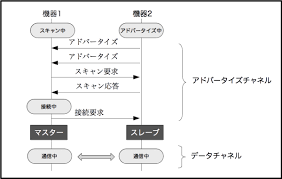
\includegraphics[width=10cm]{figures/ble_event.png}
    \caption{BLEの通信フロー}
    \label{fig:ble_event_flow}
    \end{center}
\end{figure}

\begin{table}[]
    \caption{LE packet structure}\label{fig:BLE_LE_PACKET_STRUCTURE}
    \centering
    \begin{tabular}{|c|c|c|c|}
    \hline
    \begin{tabular}[c]{@{}c@{}}Preamble\\ (1 octet)\end{tabular} & \begin{tabular}[c]{@{}c@{}}Access Address\\ (4 octets)\end{tabular} & \begin{tabular}[c]{@{}c@{}}PDU\\ (2 to 39 octets)\end{tabular} & \begin{tabular}[c]{@{}c@{}}CRC\\ (3 octets)\end{tabular} \\ \hline
    \end{tabular}
\end{table}

\begin{table}[]
    \caption{Advertising Channel PDU}\label{fig:BLE_ADV_CHANNEL_PDU}
    \centering
    \begin{tabular}{|c|c|c|}
    \hline
    \begin{tabular}[c]{@{}c@{}}Header\\ (2 octets)\end{tabular} & \begin{tabular}[c]{@{}c@{}}Advertiser's Address\\ (6 octets)\end{tabular} & \begin{tabular}[c]{@{}c@{}}Advertiser's Data\\ up to 31 octets\end{tabular} \\ \hline
    \end{tabular}
\end{table}